\documentclass[aspectratio=169]{beamer}
\geometry{paperwidth=160mm,paperheight=100mm}
\usepackage{beamerthemesidebar}
\usepackage{hyperref}
\usepackage{color}
\usepackage{multimedia}
\usepackage{colortbl}
\usepackage{amsmath}
\usepackage{empheq}
\usepackage{cancel}
\usepackage{amssymb}
\usepackage{amsfonts}
\usepackage{lipsum}
\usepackage{tcolorbox}
\usepackage{tabularx}
\usepackage{caption}
\usepackage{bm}

\setbeamersize{sidebar width right=0pt}
\setbeamertemplate{footline}[frame number]
%
\definecolor{orange}{RGB}{250,167,12}
\definecolor{yellow}{RGB}{246,250,12}
\definecolor{green}{RGB}{128,238,1}
\definecolor{black}{RGB}{0,0,0}
\definecolor{blue}{RGB}{0,0,255}
\definecolor{red}{RGB}{255,0,0}
\definecolor{sepia}{RGB}{94,38,18}
\newcommand{\ve}[1]{{\rm\bf {#1}}}
\newcommand{\q}[1]{\textcolor{blue}{#1}}
\newcommand{\blue}[1]{\textcolor{blue}{#1}}
\newcommand{\sepia}[1]{\textcolor{sepia}{#1}}
\newcommand{\red}[1]{\textcolor{red}{#1}}
\newcommand{\green}[1]{\textcolor{green}{#1}}
\newcommand{\yellow}[1]{\textcolor{yellow}{#1}}
\newcommand{\orange}[1]{\textcolor{orange}{#1}}
\definecolor{burlywood}{RGB}{255,211,155}
\definecolor{chocolate}{RGB}{255,127,36}
\definecolor{tan}{RGB}{210,180,140}
%
\def\onethird{{\textstyle{1\over3}}}
\def\twothirds{{\textstyle{2\over3}}}
\def\fourthirds{{\textstyle{4\over3}}}
\def\fivethirds{{\textstyle{5\over3}}}
\def\onehalf{{\textstyle{1\over2}}}
\def\threehalfs{{\textstyle{3\over2}}}
%
\newcommand{\pd}{\partial}
\newcommand{\aMLT}{\alpha_{\rm MLT}}
\newcommand{\Fconv}{F_{\rm conv}}
\newcommand{\Frad}{F_{\rm rad}}
\newcommand{\Ftot}{F_{\rm tot}}
\newcommand{\Hp}{H_p}
\newcommand{\prad}{p_{\rm rad}}
\newcommand{\pgas}{p_{\rm gas}}
\newcommand{\TTc}{T_{\rm c}}
\newcommand{\rhoc}{\rho_{\rm c}}
\newcommand{\Teff}{T_{\rm eff}}
\newcommand{\Fstar}{F_\star}
\newcommand{\pstar}{p_\star}
\newcommand{\Pstar}{P_\star}
\newcommand{\Rstar}{R_\star}
\newcommand{\rhostar}{\rho_\star}
\newcommand{\Tstar}{T_\star}
\newcommand{\eee}{\bm{e}}
\newcommand{\kkk}{\bm{k}}
\newcommand{\rrr}{\bm{r}}
\newcommand{\uuu}{\bm{u}}
\newcommand{\FFF}{\bm{F}}
\newcommand{\gggg}{\bm{g}}
%
\title{Theoretical Astrophysics I: Physics of Sun and Stars\\
Lecture 11: Solar oscillations and helioseismology}
\author{\texorpdfstring{\sepia{Petri K\"{a}pyl\"{a} Ivan Mili\'{c}}\newline\blue{\url{pkapyla, milic@leibniz-kis.de}}}{}}
\institute{Institut f\"ur Sonnenphysik - KIS, Freiburg}
\date{\today}
%
\begin{document}
\frame{\titlepage}


\section{Solar oscillations}
%
%
\frame{
\frametitle{Pulsating stars - Cursory introductions}
\begin{minipage}{0.54\linewidth}
\begin{itemize}
\item A zoo of oscillating stars have been observed.
\item Many (but not all) of these occur in stars that have left the
  main sequence (giant and white dwarf phases).
\item Some of these stars (e.g.\ the Cepheids) are very important in
  astrophysical distance determinations as \emph{standard
  candles}. Ivan will talk more about these next week.
\item Here we will concentrate only on solar like oscillations.
\end{itemize}
\end{minipage}
\begin{minipage}{0.45\linewidth}
\begin{figure}
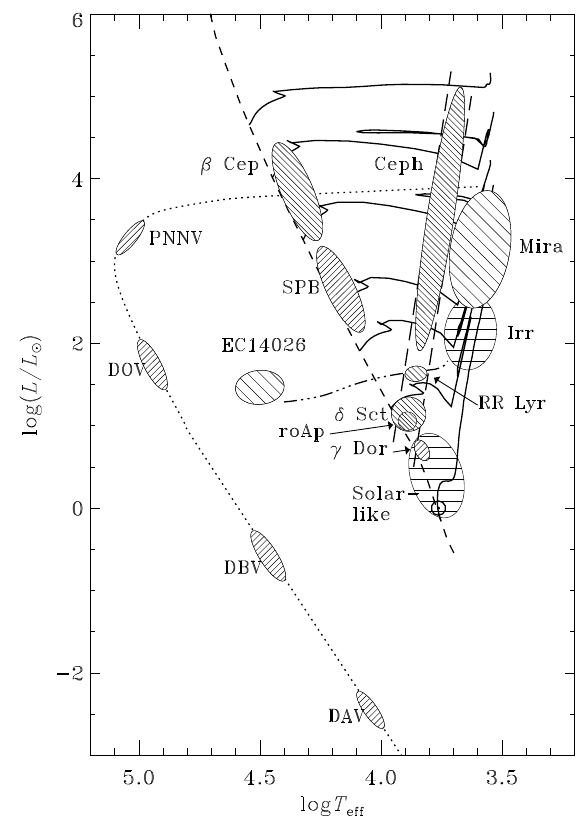
\includegraphics[width=4.5cm]{figures/oscillations_JCD.png}
\caption*{Credits: J{\o}rgen Christensen-Dalsgaard, lecture notes on
  stellar oscillations.}
\end{figure}
\end{minipage}
}
%
\frame{
\frametitle{Solar oscillations}
\begin{itemize}
\item The photosphere of the Sun supports so-called 5 minute
  oscillations. These were discovered in the 1960s.
\item In 1974-75 it was discovered that these oscillations have a
  spectrum of discrete frequencies.
\item A wide spectrum of oscillations in the range $2\ldots 15$
  minutes are also observed.
\item These are identified as acoustic (sound) waves where the
  pressure force is the restoring force. Therefore we refer to these
  as p modes.
\item Another type of waves where the gravitational force (gravity
  waves or g modes) is the restoring force occur in radiative layers.
\item There is also a surface gravity wave (f mode) that is observable.
\item The discrete spectrum of the p modes is the result of reflecting
  boundaries and therefore these waves can tell us about the interior
  structure of the Sun.
\end{itemize}
}
%
%
\frame{
\frametitle{Equations of hydrodynamics}
\begin{itemize}
\item Continuity (mass conservation):
 \begin{equation}
   \frac{\pd \rho}{\pd t} + \bm\nabla\bm\cdot (\rho\uuu) = 0.
 \end{equation}
\item Motion (momentum conservation):
 \begin{equation}
   \rho \frac{\pd \uuu}{\pd t} + \rho\uuu \bm\cdot \bm\nabla\uuu = -
   \bm\nabla p + \rho\gggg.
 \end{equation}
\item Gravity:
 \begin{equation}
   \gggg =  - \bm\nabla \Phi, \ \ \ \nabla^2 \Phi = 4\pi G \rho.
 \end{equation}
\item Energy conservation:
 \begin{equation}
   \rho \frac{{\rm d} q}{{\rm d} t} = \frac{1}{\gamma_3 - 1}\left(\frac{{\rm d}p}{{\rm d}t} - \gamma_1\frac{p}{\rho}\frac{{\rm d}\rho}{{\rm d}t} \right) = \rho \epsilon - \bm\nabla \bm\cdot \FFF.
 \end{equation}
\end{itemize}
}
%
%
\frame{
\frametitle{Equations of hydrodynamics}
\begin{itemize}
\item The different $\gamma$s are defined via
  \begin{equation}
    \gamma_1 = \left(\frac{\pd \ln p}{\pd \ln \rho}\right)_{\rm ad},\ \ \ \frac{\gamma_2 -1}{\gamma_2} = \left(\frac{\pd \ln T}{\pd \ln p}\right)_{\rm ad},\ \ \ \gamma_3 -1 = \left(\frac{\pd \ln T}{\pd \ln \rho}\right)_{\rm ad}.
  \end{equation}
\item For ideal gas law:
  \begin{equation}
    \gamma_1 = \gamma_2 = \gamma_3 \equiv \gamma = \fivethirds.
  \end{equation}
\item Assume small perturbations (primes) around an equilibrium
  (subscript 0). The latter is:
  \begin{eqnarray}
    \uuu_0 &=& 0, \ \ \bm\nabla p_0 = \rho_0 \gggg_0,\ \ 
    \gggg_0 = - \frac{Gm_0}{r^2}\hat{\eee}_r, \\
    \rho_0 \epsilon_0 &=& \bm\nabla\bm\cdot\FFF_0 = \frac{1}{r^2} \frac{\rm d}{{\rm d}r}(r^2 F_0) = \frac{1}{4\pi r^2} \frac{{\rm d}L_0}{{\rm d}r}.
  \end{eqnarray}
\item Perturbations:
  \begin{equation}
    p(\rrr,t) = p_0(\rrr,t) + p'(\rrr,t),\ \ \mbox{etc.},\ \ \uuu' = \frac{\pd \delta\rrr}{\pd t}.
  \end{equation}
\end{itemize}
}
%
%
\frame{
\frametitle{Linearized equations}
\begin{itemize}
\item Continuity:
  \begin{equation}
   \rho' + \bm\nabla\bm\cdot (\rho_0 \delta\rrr) = 0.\label{equ:linco}
  \end{equation}
\item Motion (momentum conservation):
 \begin{equation}
   \rho_0 \frac{\pd^2 \delta\rrr}{\pd t^2} = \rho_0 \frac{\pd \uuu}{\pd t} = 
   -\bm\nabla p' + \rho_0 \gggg' + \rho'\gggg_0.
 \end{equation}
\item Poisson equation:
  \begin{equation}
    \nabla^2 \Phi' = 4\pi G \rho', \ \ \gggg' = -\bm\nabla \Phi'.
  \end{equation}
\item Adiabaticity:
  \begin{equation}
    p' = \gamma_{1,0} \frac{p_0}{\rho_0} \rho'.\label{equ:linad}
  \end{equation}
\end{itemize}
}
%
%
\frame{
\frametitle{Examples of simple waves: Acoustic waves (p modes)}
\begin{itemize}
\item \emph{Acoustic waves}: Consider a spatially homogeneous case
  where the derivatives of the 0-quantities vanish.
\item This implies vanishing $\gggg_0$ which does not happen in
  reality but is a fair approximation if the 0-state varies slowly in
  comparison to the perturbations.
\item For rapid perturbations oppositely signed $\rho'$ nearly cancel
  and hence $\Phi'$ is small.
\item Finally, the adiabatic approximation is assumed.
\item Equation of motion:
  \begin{equation}
    \rho_0 \frac{\pd^2 \delta\rrr}{\pd t^2} = - \bm\nabla p',\ \  \xRightarrow[\text{ }]{\text{$\bm\nabla\bm\cdot (\ldots)$}}\ \ \rho_0 \frac{\pd^2}{\pd t^2} (\bm\nabla\bm\cdot \delta\rrr) = - \nabla^2 p'.
  \end{equation}
\end{itemize}
}
%
%
\frame{
\frametitle{Examples of simple waves: Acoustic waves (p modes)}
\begin{itemize}
\item Use Eqs.~(\ref{equ:linco}) and (\ref{equ:linad}) to eliminate
  $\delta\rrr$ and $p'$ gives
  \begin{equation}
    -\rho_0 \frac{\pd^2}{\pd t^2} (\bm\nabla\bm\cdot \delta\rrr) = \frac{\pd^2 \rho'}{\pd t^2} = \gamma_{1,0} \frac{p_0}{\rho_0} \nabla^2 \rho' \equiv c_0^2 \nabla^2 \rho',\label{equ:sound}
  \end{equation}
\item where
  \begin{equation}
    c_0^2 = \gamma_{1,0} \frac{p_0}{\rho_0},
  \end{equation}
  has the unit of squared velocity. We identify Eq.~(\ref{equ:sound})
  as a wave equation and $c_0^2$ as the \emph{speed of sound}.
\item Solutions are in the form of plance waves:
  \begin{equation}
    \rho' = a \exp[i (\kkk\bm\cdot\rrr - \omega t)].\label{equ:plane}
  \end{equation}
\item (The physical solution is the \emph{real part} of the complex
  solution.)
\end{itemize}
}
%
%
\frame{
\frametitle{Examples of simple waves: Acoustic waves (p modes)}
\begin{itemize}
\item Substituting (\ref{equ:plane}) back to Eq.~(\ref{equ:sound})
  yields the \emph{dispersion relation} of sound waves:
  \begin{equation}
    \omega^2 = c_0^2 |\kkk|^2.
  \end{equation}
\item \blue{What can you conclude about sound waves based on this
  equation?}
\end{itemize}
}
%
%
\frame{
\frametitle{Examples of simple waves: Acoustic waves (p modes)}
\begin{itemize}
\item Substituting (\ref{equ:plane}) back to Eq.~(\ref{equ:sound})
  yields the \emph{dispersion relation} of sound waves:
  \begin{equation}
    \omega^2 = c_0^2 |\kkk|^2.
  \end{equation}
\item \blue{What can you conclude about sound waves based on this
  equation?}
\item The permissible frequencies depend on the wavenumber,
  i.e.\ spatial scale of the cavity where the sound waves
  propagate. In stars this is bounded by the size of the star. The
  speed of sound also varies internally such that the combination of
  $c_0$ and $|\kkk|$ determines the frequencies.
\item For an ideal gas the squared speed of sound is:
  \begin{equation}
    c_0^2 = \gamma \frac{p_0}{\rho_0} = \gamma \frac{\cal R}{\mu} T_0 \propto \frac{T_0}{\mu}. 
  \end{equation}
\item With a suitable choice of phases the (real parts) of solutions
  read:
  \begin{eqnarray}
    & \rho' = a \cos(\kkk\bm\cdot\rrr - \omega t), & \\
    & p' = c_0^2 a \cos(\kkk\bm\cdot\rrr - \omega t), & \\
    & \delta\rrr = \frac{c_0^2}{\rho_0 \omega^2} a \cos\left(\kkk\bm\cdot\rrr - \omega t + \frac{\pi}{2}\right)\kkk. &
  \end{eqnarray}
\end{itemize}
}
%
%
\frame{
\frametitle{Examples of simple waves: Internal gravity waves (g modes)}
\begin{itemize}
\item Waves that exist in convectively stable regions instead of
  convection (radiative interior of the Sun).
\item Tutorials\ldots
\end{itemize}
}
%
%
\frame{
\frametitle{Examples of simple waves: Surface gravity waves (f mode)}
\begin{itemize}
\item Surface gravity waves occur at the interface of between two
  media where the gravity and buoyancy both try to restore equilibrium
  (e.g., waves in the sea).
\item Tutorials\ldots
\end{itemize}
}
%
%
\frame{
\frametitle{Oscillations in the Sun}
\begin{itemize}
\item As already alluded to, waves in the Sun are low amplitude and
  can therefore be treated as linear perturbations. Their periods are
  much shorter than the thermal timescale such that the adiabatic
  approximation is valid.
\item The oscillation modes are thought to be excited stochastically
  by convective motions. The damping of modes is also due to
  convective flows and turbulent motions. Therefore the oscillations
  occur on a broad frequency spectrum.
\item \blue{If the driving is stochastic why doesn't destructive
  interference wipe out the waves?}
\end{itemize}
}
%
%
\frame{
\frametitle{Oscillations in the Sun}
\begin{itemize}
\item As already alluded to, waves in the Sun are low amplitude and
  can therefore be treated as linear perturbations. Their periods are
  much shorter than the thermal timescale such that the adiabatic
  approximation is valid.
\item The oscillation modes are thought to be excited stochastically
  by convective motions. The damping of modes is also due to
  convective flows and turbulent motions. Therefore the oscillations
  occur on a broad frequency spectrum.
\item \blue{If the driving is stochastic why doesn't destructive
  interference wipe out the waves?}
\item The observed waves are \emph{standing waves} of the
  \emph{resonant modes}.
\item The amplitudes of the modes are determined by an equilibrium
  between energy supply and damping.
\end{itemize}
}
%
\frame{
\frametitle{Oscillations in the Sun: Dopplergram}
\begin{minipage}{0.495\linewidth}
\begin{itemize}
\item Dopplergram of the Sun: radial velocity signal from convection
  and waves.
\item These can be obtained from the full disk or from high-resolution
  observations of smaller patches of the Sun.
\item Here we discuss only global modes and full disk observations.
\end{itemize}
\end{minipage}
\begin{minipage}{0.495\linewidth}
\begin{figure}
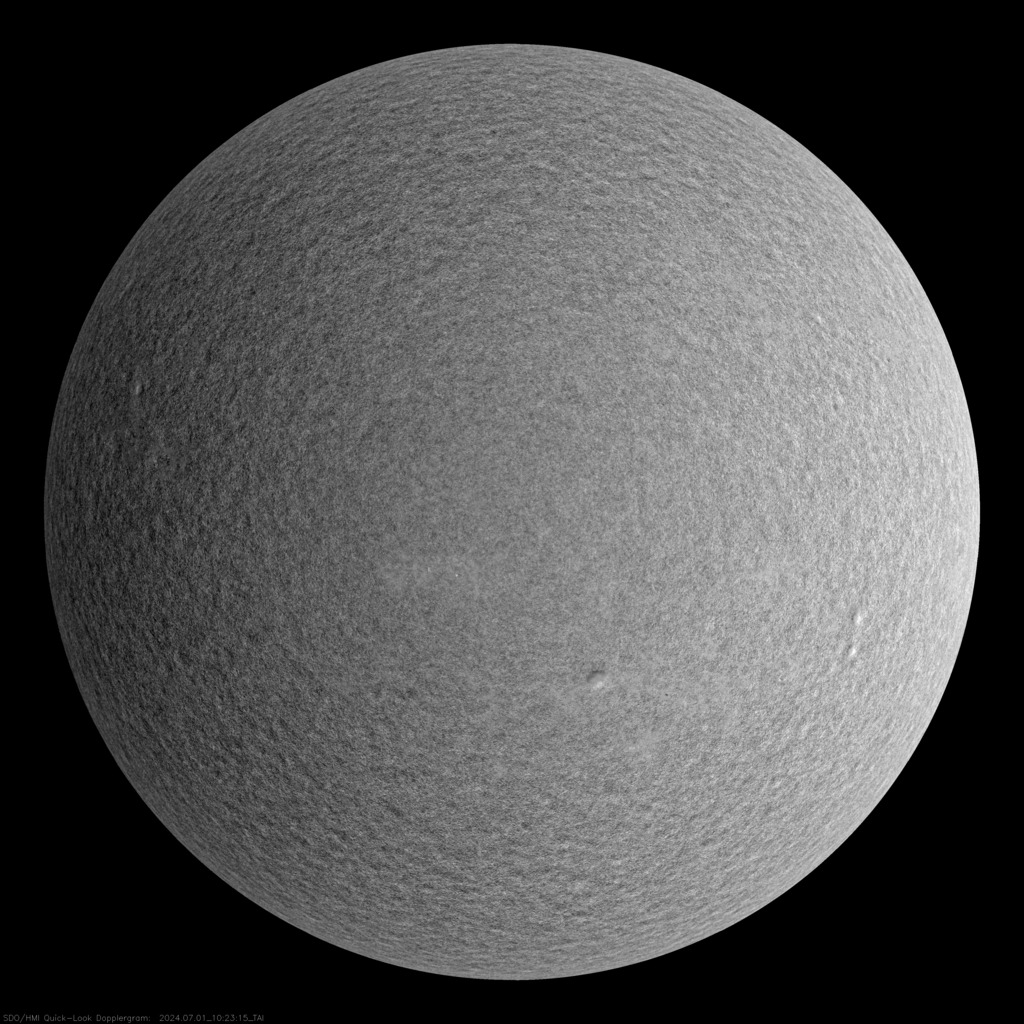
\includegraphics[width=6cm]{figures/latest_1024_HMID.jpg}
\caption*{Credit: Solar Dynamics Observatory}
\end{figure}
\end{minipage}
}
%
%
\frame{
\frametitle{Spherical Harmonics}
\begin{minipage}{0.495\linewidth}
\begin{itemize}
\item Global analysis is done by expanding the data in terms of
  \emph{spherical harmonics} $Y_\ell^m(\theta,\phi)$:
  \begin{equation}
    f(r,\theta,\phi,t) = \sum_{\ell=0}^\infty \sum_{m=-\ell}^\ell f_\ell^m(t) r^\ell Y_\ell^m(\theta,\phi),
  \end{equation}
  where $f_\ell^m$ is a scalar coefficient and
  \begin{equation}
    Y_\ell^m(\theta,\phi) = C(m,\ell) P_\ell^m (\cos\theta) e^{im\phi},
  \end{equation}
  where $C(m,\ell)$ is a normalization factor and $P_\ell^m$ are the
  associated Legendre polynomials.
\end{itemize}
\end{minipage}
\begin{minipage}{0.495\linewidth}
\begin{figure}
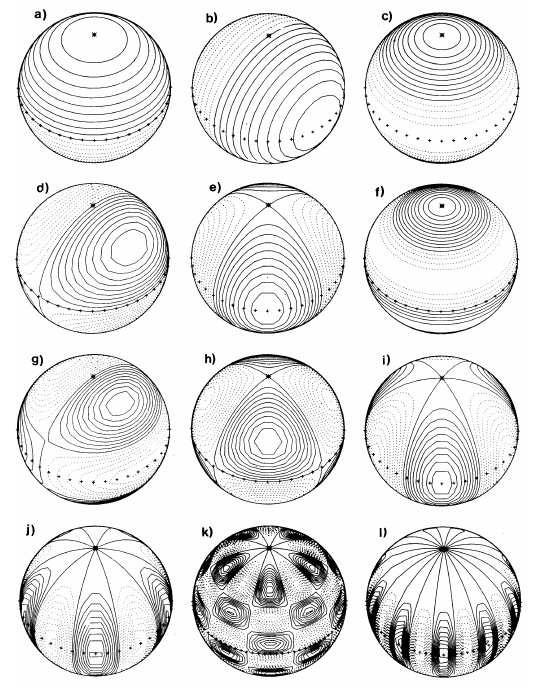
\includegraphics[width=5.5cm]{figures/spherical_harmonics_JCD.png}
\caption*{Credits: Christensen-Dalsgaard, Lecture notes on stellar oscillations}
\end{figure}
\end{minipage}
}
%
%
\frame{
\frametitle{Fourier transform}
\begin{itemize}
\item Energy density:
  \begin{equation}
    E \equiv \int_{-\infty}^\infty |x(t)|^2 dt.
  \end{equation}
\item Parseval's theorem
  \begin{equation}
    \int_{-\infty}^\infty |x(t)|^2 dt = \int_{-\infty}^\infty |\hat{x}(\omega)|^2 dt,
  \end{equation}
  where
  \begin{equation}
    \hat{x}(\omega) \equiv \int_{-\infty}^\infty e^{-i\omega t} x(t)dt,
  \end{equation}
  is the \emph{Fourier transform}.
\item The \emph{spectral energy density} is given by:
  \begin{equation}
    E(\omega) = |\hat{x}(\omega)|^2,
  \end{equation}
  which can be used to detect periodic signals.
\end{itemize}
}
%
%
\frame{
\frametitle{Fourier transform}
\begin{itemize}
\item Consider a signal $x(t) = \sin(\omega_0 t)$ and its Fourier
  transform:
  \begin{equation}
    \hat{x}(\omega) = \frac{\pi}{i} [\delta(\omega - \omega_0) - \delta(\omega + \omega_0)].
  \end{equation}
\end{itemize}
\begin{figure}
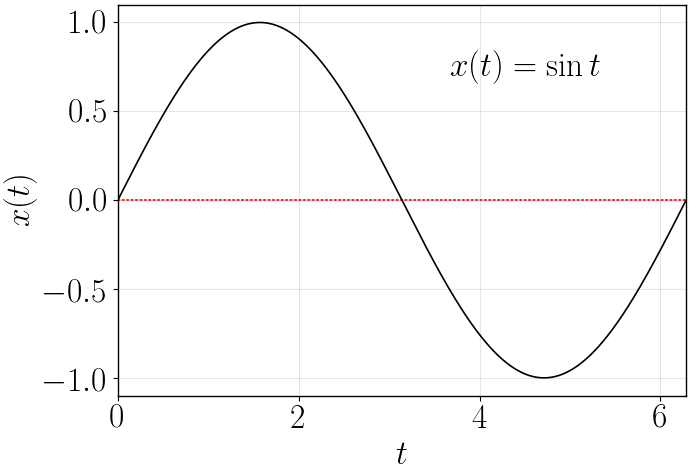
\includegraphics[width=7.5cm]{figures/sint.png}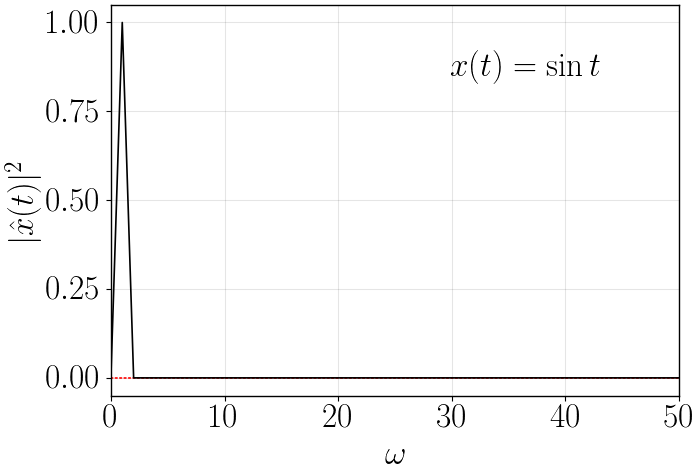
\includegraphics[width=7.5cm]{figures/psint.png}
\caption*{Function $x$ and its \emph{power spectrum}.}
\end{figure}
}
%
%
\frame{
\frametitle{Fourier transform}
\begin{itemize}
\item Consider now a signal:
  \begin{equation}
  x(t) = \sin(\omega t) + \onehalf \sin (3 t) + 3 \sin(30 t).
  \end{equation}
\end{itemize}
\begin{figure}
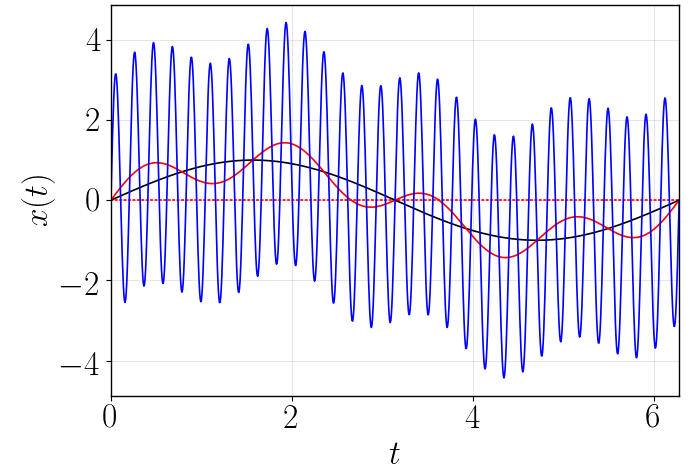
\includegraphics[width=7.5cm]{figures/sint3.png}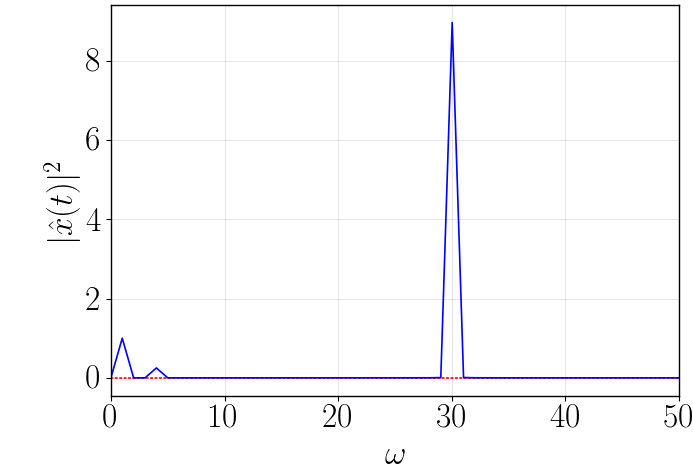
\includegraphics[width=7.5cm]{figures/psint3.png}
\caption*{Function $x$ and its \emph{power spectrum}.}
\end{figure}
}
%
%
\frame{
\frametitle{Fourier transform}
\begin{itemize}
\item Consider now a signal:
  \begin{equation}
  x(t) = \sin(\omega t) + \onehalf \sin (3 t) + 3 \sin(30 t) + \mbox{noise}.
  \end{equation}
\end{itemize}
\begin{figure}
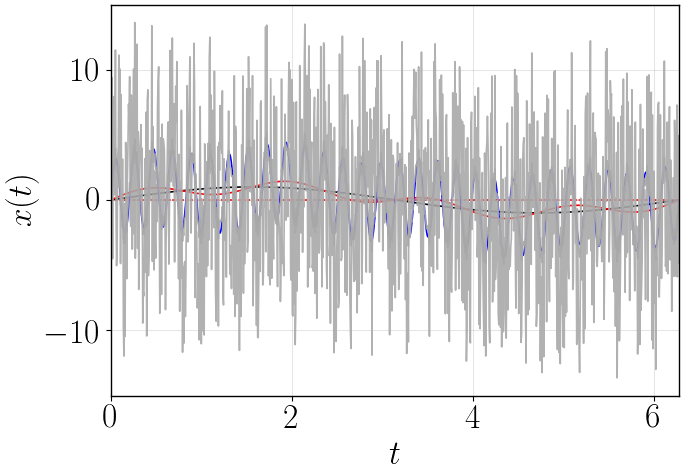
\includegraphics[width=7.5cm]{figures/sint4.png}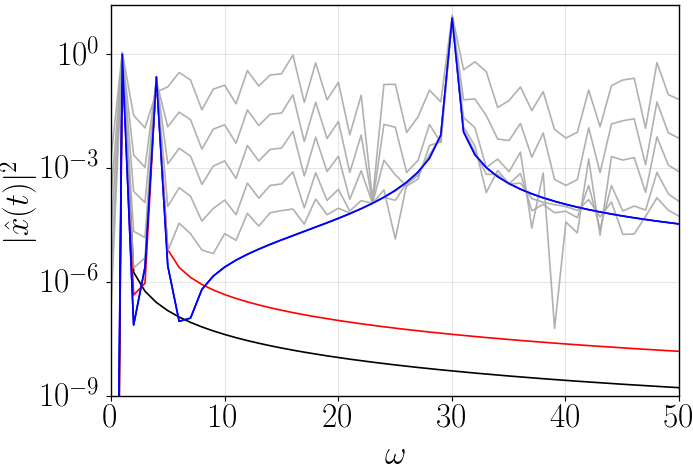
\includegraphics[width=7.5cm]{figures/psint4.png}
\caption*{Function $x$ and its \emph{power spectrum}.}
\end{figure}
}
%
%
\frame{
\frametitle{Oscillations in the Sun: Experimental verification}
\begin{minipage}{0.495\linewidth}
\begin{figure}
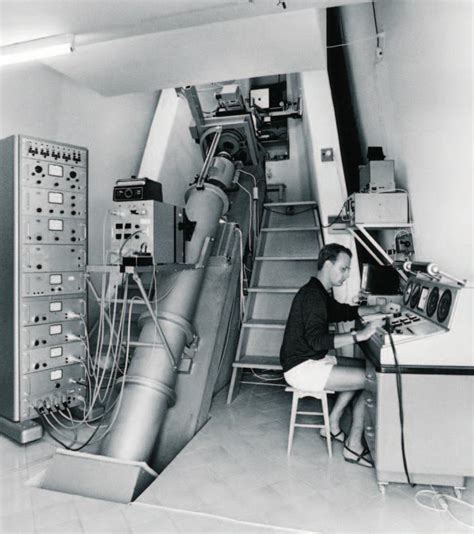
\includegraphics[width=6cm]{figures/Franz-Ludwig_Deubner.jpeg}
\caption*{Franz-Ludwig Deubner at Capri, 1974.}
\end{figure}
\end{minipage}
\begin{minipage}{0.495\linewidth}
\begin{figure}
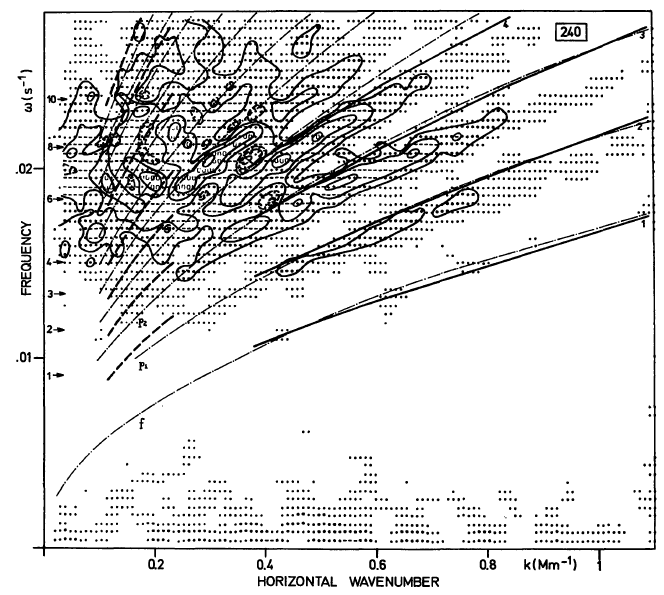
\includegraphics[width=7.5cm]{figures/Deubner_1975_modes.png}
\caption*{Credits: Deubner (1975), A\&A, {\bf 44}, 371.}
\end{figure}
\end{minipage}
}
%
%
\frame{
\frametitle{Oscillations in the Sun}
\begin{minipage}{0.495\linewidth}
\begin{itemize}
\item Modern $k$-$\omega$ diagram shows many ridges that can be
  identified as p modes.
\item Figure on the right shows the power spectrum of medium angular
  degree $\ell$ solar oscillations, computed for 144 days of data from
  the MDI instrument aboard SOHO.
\item Long time series is needed to resolve the ``ridges'' (the longer
  the better).
\item Preferably the time series should not have gaps $\Rightarrow$
  continuous observations from space (SOHO, SDO) or from networks of
  telescopes around the world (e.g. BISON, GONG).
\end{itemize}
\end{minipage}
\begin{minipage}{0.495\linewidth}
\begin{figure}
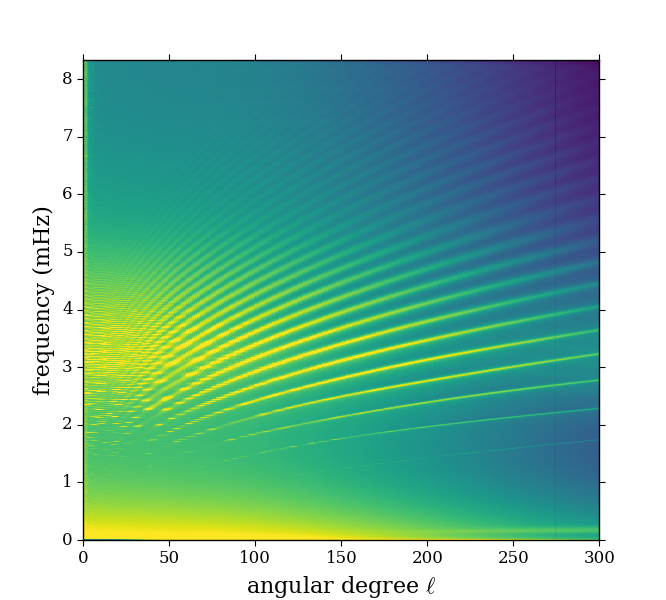
\includegraphics[width=7.5cm]{figures/MDI_medium_angular_degree_power_spectrum.png}
\caption*{Credits: SOHO/MDI.}
\end{figure}
\end{minipage}
}
%
%
\frame{
\frametitle{Oscillations in the Sun: Mode trapping}
\begin{itemize}
\item Modes with different spherical harmonic degree $\ell$ and
  frequency $\nu$ are \emph{trapped} at different depths.
\end{itemize}
\begin{minipage}{0.495\linewidth}
\begin{figure}
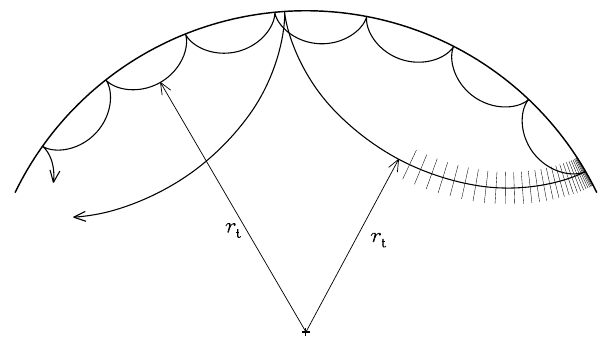
\includegraphics[width=7cm]{figures/acoustic_waves_JCD.png}
\caption*{Credits: Christensen-Dalsgaard, Lecture notes on stellar oscillations}
\end{figure}
\end{minipage}
\begin{minipage}{0.495\linewidth}
\begin{figure}
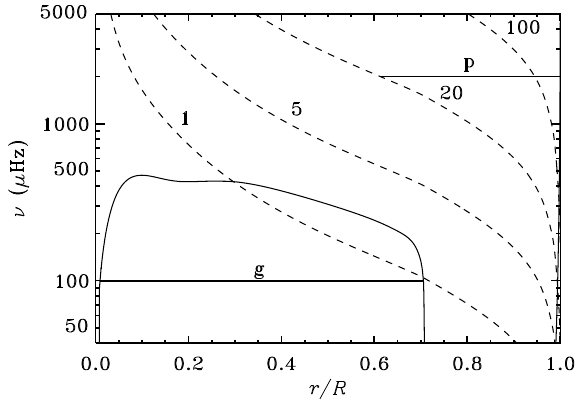
\includegraphics[width=7.5cm]{figures/mode_trapping_JCD.png}
\caption*{Credits: Christensen-Dalsgaard, Lecture notes on stellar
  oscillations. Numbers refer to $\ell$.}
\end{figure}
\end{minipage}
}
%
%
\frame{
\frametitle{Oscillations in the Sun vs. in simulations}
\begin{minipage}{0.495\linewidth}
\begin{itemize}
\item Modes in solar surface convection simulations agree well with
  solar observations.
\item This supports the idea that the oscillations are excited by
  convection.
\item Simulations can be used to probe effects of magnetic fields,
  convection zone structure, etc. on oscillation modes.
\end{itemize}
\end{minipage}
\begin{minipage}{0.495\linewidth}
\begin{figure}
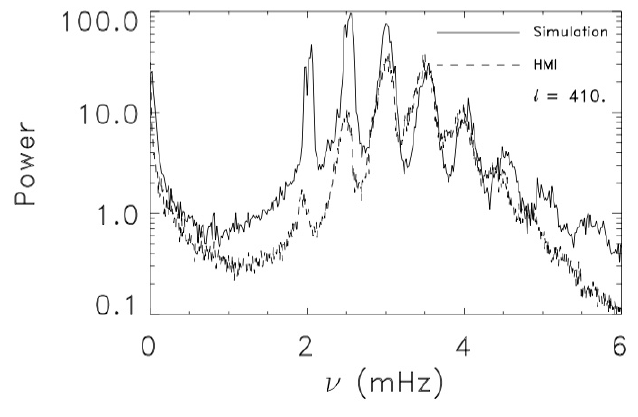
\includegraphics[width=7.5cm]{figures/Stein_2024_oscillations.png}
\caption*{Credits: Stein et al. (2024), arXiv:2405.02483}
\end{figure}
\end{minipage}
}
%
%
\frame{
\frametitle{How good are solar and stellar structure models?}
\begin{minipage}{0.495\linewidth}
\begin{itemize}
\item Oscillation frequencies from a \emph{model Sun}, i.e., from a
  model that is a solution of the stellar structure equations for the
  solar age.
\end{itemize}
\end{minipage}
\begin{minipage}{0.495\linewidth}
\begin{figure}
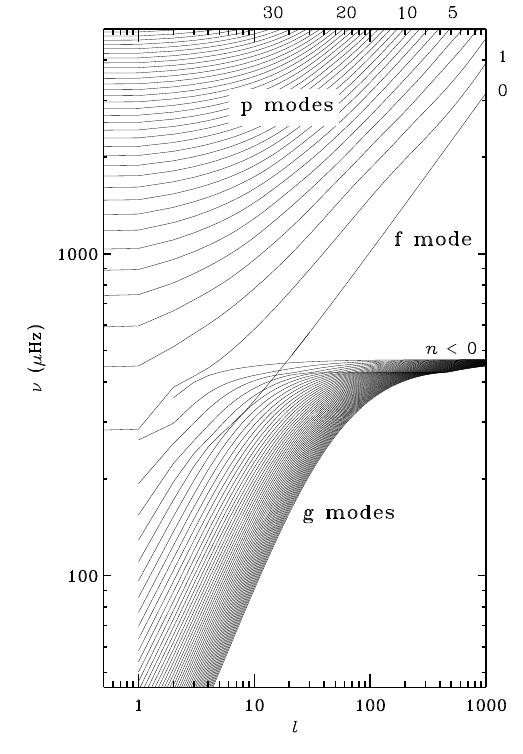
\includegraphics[width=5cm]{figures/modes_in_model_sun_JCD.png}
\caption*{Credits: Christensen-Dalsgaard, Lecture notes on stellar oscillations}
\end{figure}
\end{minipage}
}
%
%
\frame{
\frametitle{Duvall's law and sound speed inversion}
\begin{itemize}
\item Duvall's law (Duvall 1982, Nature, 300, 242):
  \begin{equation}
    F\left(\frac{\omega}{L} \right) = \int_{r_t}^R \left(1 - \frac{L^2 c^2}{\omega^2 r^2} \right)^{1/2} \frac{{\rm d}r}{c} = \frac{[n+\alpha(\omega)]\pi}{\omega},\ \ \ L = \ell+\onehalf.
  \end{equation}
\item This equation is an implicit equation for $c$ which is the sound
  speed and allows to solve for it \emph{without resorting to any
  model of the solar interior}.
\end{itemize}
\begin{figure}
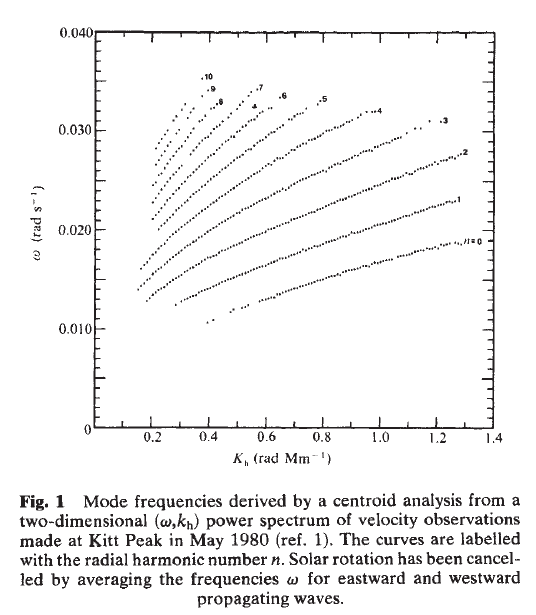
\includegraphics[width=5cm]{figures/Duvall-law1.png}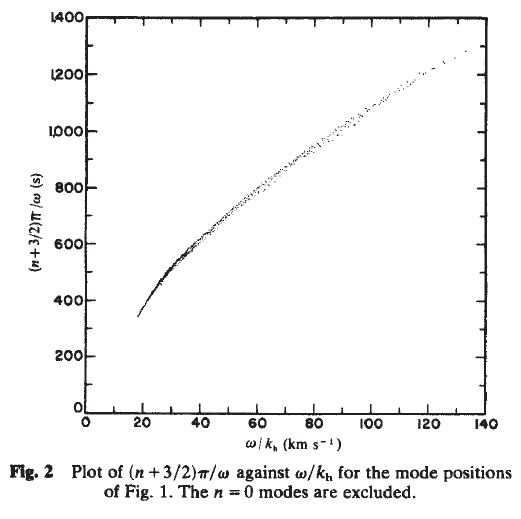
\includegraphics[width=5cm]{figures/Duvall-law2.png}
\caption*{Credits: Duvall (1982).}
\end{figure}
}
%
%
\frame{
\frametitle{How good are solar and stellar structure models?}
\begin{minipage}{0.495\linewidth}
\begin{itemize}
\item Compare sound speed profile from helioseismology to that from a
  standard solar model.
\item \blue{How well do you think the model fares?}
\end{itemize}
\end{minipage}
\begin{minipage}{0.495\linewidth}
%\begin{figure}
%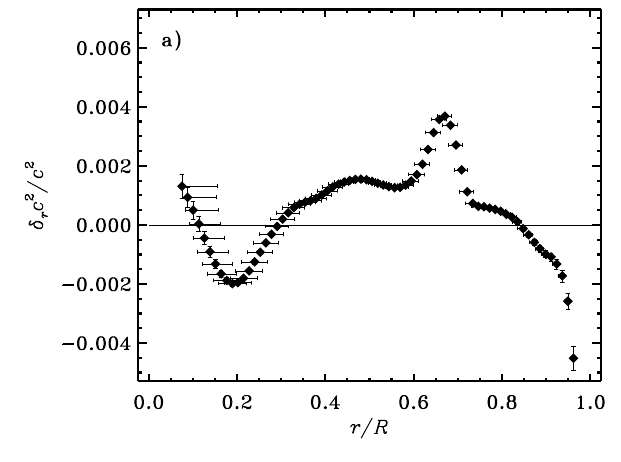
\includegraphics[width=7.5cm]{figures/sound_speed_difference.png}
%\caption*{Credits: Basu et al. (1996)}
%\end{figure}
\end{minipage}
}
%
%
\frame{
\frametitle{How good are solar and stellar structure models?}
\begin{minipage}{0.495\linewidth}
\begin{itemize}
\item Compare sound speed profile from helioseismology to that from a
  standard solar model.
\item \blue{How well do you think the model fares?}
\item Current solar models (solving the full set of stellar structure
  equations) reproduces the squared sound speed profile within 0.4 per
  cent.
\item \blue{What are the most significant sources of the discrepancy?}
\end{itemize}
\end{minipage}
\begin{minipage}{0.495\linewidth}
\begin{figure}
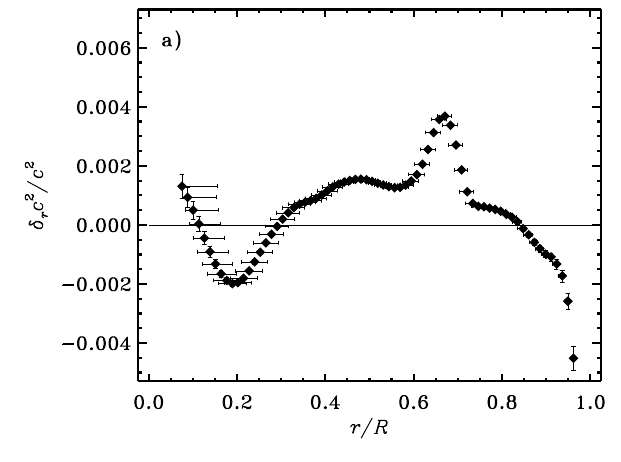
\includegraphics[width=7.5cm]{figures/sound_speed_difference.png}
\caption*{Credits: Basu et al. (1996)}
\end{figure}
\end{minipage}
}
%
%
\frame{
\frametitle{How good are solar and stellar structure models?}
\begin{minipage}{0.495\linewidth}
\begin{itemize}
\item Compare sound speed profile from helioseismology to that from a
  standard solar model.
\item \blue{How well do you think the model fares?}
\item Current solar models (solving the full set of stellar structure
  equations) reproduces the squared sound speed profile within 0.4 per
  cent.
\item \blue{What are the most significant sources of the discrepancy?}
\item Lack of data to probe the center, problems with parameterization
  of convection at the base and near the surface of the convection
  zone.
\end{itemize}
\end{minipage}
\begin{minipage}{0.495\linewidth}
\begin{figure}
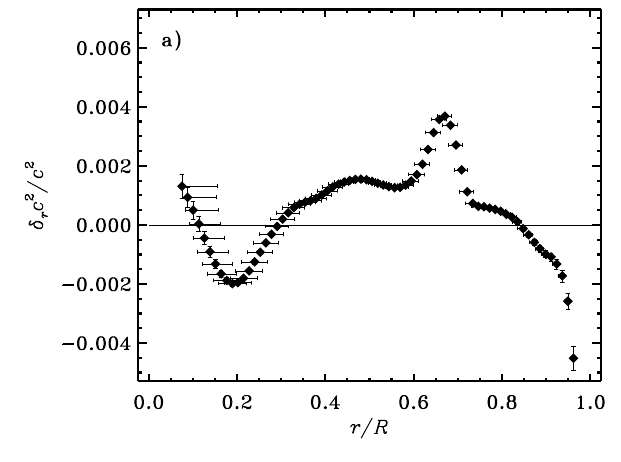
\includegraphics[width=7.5cm]{figures/sound_speed_difference.png}
\caption*{Credits: Basu et al. (1996)}
\end{figure}
\end{minipage}
}
%
%
\frame{
\frametitle{Frequency splitting}
\begin{minipage}{0.495\linewidth}
\begin{itemize}
\item Standing wave results from two waves travelling in opposite
  directions between two nodes.
\item In a rotating sytem waves travelling to opposite directions are
  advected by the flow.
\item Hence there will be a Doppler shift of frequency by the amount
  \begin{equation}
    \frac{\Delta \omega_\pm}{\omega} = \frac{u_\pm}{u_{\rm p}},
  \end{equation}
  where $u_\pm$ are the velocities of the waves and $u_{\rm p}$ is the
  phase velocity of the wave.
\item The total shift is $2\Delta\omega$ which leads the standing wave
  pattern to drift in the opposite direction of the rotation.
\end{itemize}
\end{minipage}
\begin{minipage}{0.495\linewidth}
\begin{figure}
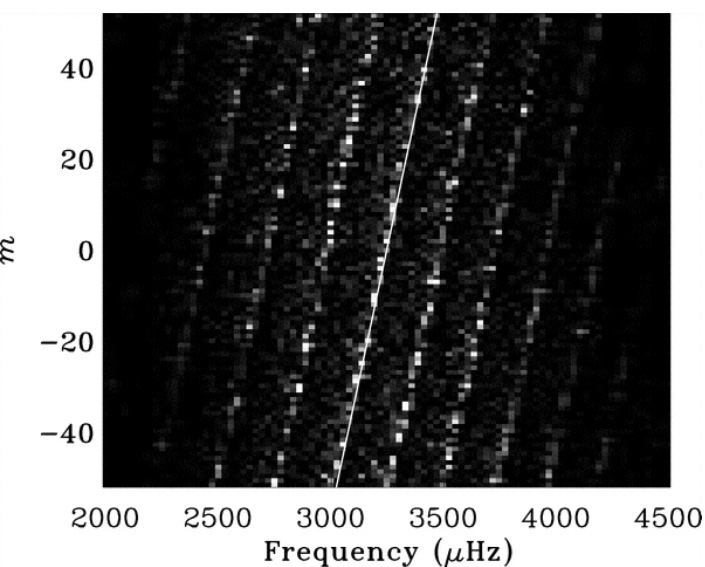
\includegraphics[width=7.5cm]{figures/freq_splitting_sun.png}
\caption*{Rotation induces a dependence on azimuthal order $m$.}
\end{figure}
\end{minipage}
}
%
%
\frame{
\frametitle{Internal rotation of the Sun}
\begin{minipage}{0.495\linewidth}
\begin{itemize}
\item The frequency splitting can be used to deduce the internal
  rotation profile of the Sun.
\item The surface differential rotation extends essentially to the
  entire convection zone.
\item Theoretical models prior to helioseismic era predicted that
  angular velocity $\Omega$ would decrease with radius. In reality the
  radial gradient is small in the bulk and large only near the
  boundaries of the convection zone.
\item This is a very important constraint for theories regarding
  stellar differential rotation and the global solar dynamo.
\end{itemize}
\end{minipage}
\begin{minipage}{0.495\linewidth}
\begin{figure}
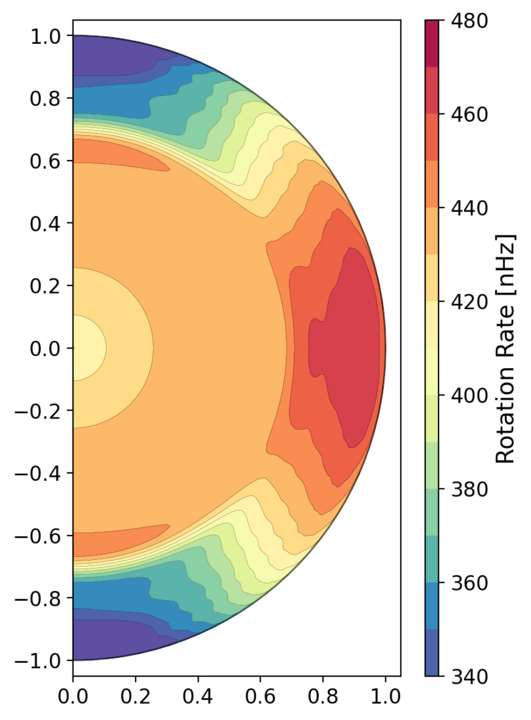
\includegraphics[width=5cm]{figures/solar_DR.png}
\caption*{Solar differential rotation from helioseismology. Credits:
  Larson \& Schou (2018).}
\end{figure}
\end{minipage}
}
%
%
\frame{
\frametitle{Internal rotation of the Sun: torsional oscillations}
\begin{itemize}
\item \emph{Torsional oscillations} (faster and slower bands of
  rotation) trace the magnetic activity (white contours).
\end{itemize}
%\begin{minipage}{0.495\linewidth}
\begin{figure}
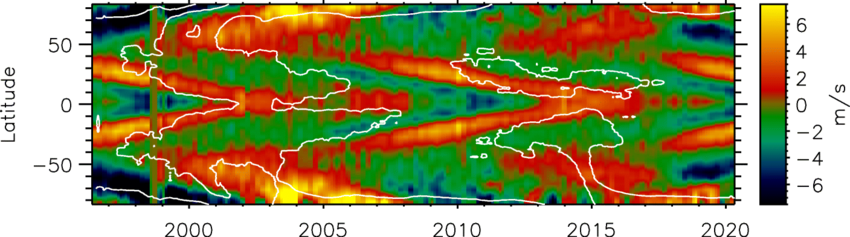
\includegraphics[width=12.5cm]{figures/solar_torsional_osc.png}
\caption*{Credits: Harra et al. (2021)}
\end{figure}
%\end{minipage}
}
%
%
\end{document}
% 

